\documentclass[a4j,10pt]{jarticle}
\title{粘性率の測定}
\author{高浜 陸生}
\date{2013年4月22日}
\usepackage[dvipdfm]{graphicx}
\newcommand{\Tabref}[1]{表~(\ref{#1})}
\newcommand{\Equref}[1]{式~(\ref{#1})}
\newcommand{\Figref}[1]{図~(\ref{#1})}
\begin{document}
\section{目的}
この実験では、細いガラス管の中に液体を吸い上げ、その降下する速度を測定することで、液体固有の物理定数である粘性率を測定する。
\section{原理}
\subsection{表面張力}
液体中の分子は周囲の分子から引力を受けて。この力の大きさは分子間の距離に依存し、分子どうしが少しの距離離れてしまうだけで0になってしまう。
このような力のことを近距離力といい、分子が受ける引力の及ぶ距離dは$10^{9}[\mathrm m]$程度までである。
この力を受けることで、分子は周囲にある他の分子からあらゆる方向に一様な引力を受ける。
しかし、分子が液体表面からd以内の距離に入ると、分子上部に引き上げる引力が弱まり不均衡になることによって、分子は内部に引き込まれるような力を受ける。
このことから、液体の表面では液体内部に向け力が働いていることを意味する。
これより、液体の自由表面を広げるには仕事が必要なことがわかる。
液体の自由表面を広げるために必要な仕事のことを表面張力という。
\\ \\ \\ \\
\begin{figure}[h]
\caption{表面積を増すには仕事を必要とする}
\label{Fig:Harigane}
\end{figure}
\\
\Figref{Fig:Harigane}に示すような針金の枠ABCD上をBCと平行を保ったまま摩擦なく滑る針金B'C'を考える。
長方形B'C'CBに液体の膜を張ると、針金B'C'には膜の面積を小さくしようとする力が働く。この力の大きさを$F$とする。
針金を$\Delta x$移動させることを考えると、膜には表と裏があるので、面積の増加は$2a\Delta x$である。
針金を動かすのに必要な仕事は表面積の増加分に比例するので、比例定数を$\gamma$とおくと、\Equref{Work}のように表される
\begin{eqnarray}
\label{Work}
F\Delta x = \gamma 2a\Delta x
\end{eqnarray}
この比例定数$\gamma$が表面張力である。$2a$は境界線の長さ($l$で表す)なので次の\Equref{Hyoumen}のような関係が導出できる。
\begin{eqnarray}
\label{Hyoumen}
F=\gamma l
\end{eqnarray}
つまり、表面張力は境界線の単位長さあたりに作用する力に等しい。以上から表面張力の単位は$J/m^{2}$とも$N/m$とも表すことができるが、一般的には$N/m$が使われる。
\subsection{粘性率}
粘性とは流体(気体と液体)中の摩擦現象である。液体の隣り合った部分が異なる速度で流れている場合に、速度の差をなくそうとして働く力が作用する現象である。
極低温の超流動状態の液体ヘリウムを除くすべての流体は粘性を有する。\\
粘性のある流体が容器の壁に接触する部分では、壁に相対的な流体の速度は0である。
自動車の車体や扇風機の羽に埃が空気の流れに飛ばされず付着しているのはこれが原因である。\\
間隔$h$で置かれた二枚の板と、その間にある流体を考える。固定された下の板に対し上の板は一定の速度$v$で運動しているとする。
この時下の板に接する流体の速度は0、上の板に接する流体の速度は$v$である。上の板と下の板の間に流れる流体の速度は\Figref{Ryusoku:1}のようになる。
この時、下の板は流れの順方向に、上の板は流れと逆方向に力を受ける。板の面積$S$が受ける力の大きさ$F$は面積$S$と速度勾配(空間的な速度変化の割合)$v/h$に比例する
($F/S \propto Sv/h$)。つまり単位面積当たりの力(応力)は
\begin{eqnarray}
\label{ouryoku}
\frac{F}{S} = \eta \frac{v}{h}
\end{eqnarray}
と表される。比例定数$\eta$を粘性率または粘性係数をよぶ。流体を板と平行な面で仮想的に分けて考えると、
この面を通して上下の液体には\Equref{ouryoku}で与えられるずれ応力が作用していることになる(面に並行な応力をずれ応力という)。
なお、粘性係数の単位は、MKS単位系では
\begin{eqnarray}
\label{nensei:tanni}
\mathrm {\frac{N/m^{2}}{(m/\mathrm s)/m} = N \cdot s \cdot m^{-2} = Pa \cdot s}
\end{eqnarray}
である。
\\ \\ \\ \\ \
\begin{figure}[h]
\begin{minipage}{.5\hsize}
\caption{互いに移動する平行な板の間の流速}
\label{Ryusoku:1}
\end{minipage}
\begin{minipage}{.5\hsize}
\caption{円形断面の管の中の流速}
\label{Ryusoku:2}
\end{minipage}
\end{figure}
\subsection{測定の原理}
円形の断面をもつ管の中を流体が乱れなく流れている場合には管内の流速は\Figref{Ryusoku:2}のようになっている。
管壁に接触する部分では流速は0であるので、管が細くなると流速は急激に小さくなる。管の半径を$a$、長さを$l$、両端での圧力差を$p_{1}-p_{2}$とすると、時間$t$の間に流れる流体の体積$V$は
\begin{eqnarray}
\label{Poiseuille}
V = \frac{\pi a^{4}(p_{1}-p_{2}}{8 \eta l}t
\end{eqnarray}
となることが知られている。\Equref{Poiseuille}をポアズイユ(Poiseuille)の法則という。管内の平均流速$v$は、\Equref{Poiseuille}における単位時間あたりの流量$V/t$を断面積で割って得られる(\Equref{Poi:r})
\begin{eqnarray}
\label{Poi:r}
v=\frac{V}{\pi a^{2}t}=\frac{a^{2}(p_{1}-p_{2})}{8 \eta l}
\end{eqnarray}
内半径$a$の細いガラス管(毛細管)を鉛直から角$\theta$だけ傾け、下端を液面にい触れさせる。このガラス管の中に液体を吸い上げ、途中に切れ目のない長い液柱を作る。管内の圧力を大気圧に戻すと、液柱の上端が
ゆっくり降下する。液体の密度$\rho$、液柱の長さを$l$とすると、液柱の質量は$\pi a^{2}l\rho$であるから、ガラス管した方向に液を押し下げようとする力は$\pi a^{2}l\rho g \cos{\theta}$である($g$は重力加速度)。
また液体表面と管壁の境界線に作用する液を引き上げようとする表面張力による力は$2\pi a \gamma$である。したがって\Equref{Poi:r}の圧力差に
\begin{eqnarray}
\label{pres:dif}
p_{1}-p_{2}=\frac{\pi a^{2}l\rho g \cos{\theta}-2\pi a \gamma}{\pi a^2}=\left(\rho g \cos{\theta} - \frac{2\gamma}{al}\right)
\end{eqnarray}
を代入し、\Equref{v-fin}を得る
\begin{eqnarray}
\label{v-fin}
v=\frac{a^2}{8 \eta}\left(\rho g \cos{\theta} - \frac{2\gamma}{al}\right)
\end{eqnarray}
この$v$が液頭の降下する速度である。降下すると液中の長さは短くなるので次第に効果速度は遅くなり、最終的に停止する。停止した際($v=0$)の液柱の長さ$l_0$は
\begin{eqnarray}
\label{l0}
l_0=\frac{2\gamma}{a\rho g \cos{\theta}}
\end{eqnarray}
である。ガラス管内で液体が表面張力によって引き上げられる現象を毛管現象という。毛管現象が認められるような細い管を毛細管と呼ぶ。
毛細管内に吸い上げた液体の上端の降下速度$v$を縦軸に、液柱の長さの逆数$1/l$を横軸にとり\Equref{v-fin}をグラフに表すと、直線が得られる。
直線が縦軸と交わる点を$v_0$、横軸と交わる点を$l_0$とすれば、$v_0$、$l_0$はそれぞれ粘性率$\eta$、表面張力$\gamma$と\Equref{eta}、\Equref{gamma}のような関係になる。
\begin{eqnarray}
\label{eta}
\eta = \frac{a^2}{8v_0}\rho g \cos{\theta}\\
\label{gamma}
\gamma = \frac{1}{2}al_0\rho g \cos{\theta}
\end{eqnarray}
\section{実験方法}
毛細管につけた目印の標線を液頭が通過する時間を測り、各区間の平均速度を求める。区間の中点を通過する速度が平均速度に等しいとみなしグラフを作成する。
グラフより$v_0$、$l_0$を求め、\Equref{eta}、\Equref{gamma}を用い粘性率と表面張力を求める。測定は水とエタノール、及びその混合溶液で行う。
\subsection{準備}
\begin{enumerate}
\item 使用する毛細管の半径と番号をメモする。
\item 毛細管には適当な間隔で標線が付いている。上のほうから1,2,3...を割り振り、下端から各標線までの長さを計測する。
\item 試料の溶液をシャーレにとり、鉛直方向から 50°~70°傾けて毛細管を立てる。傾き角$\theta$を分度器で測定する。なお、毛細管を深く浸すと\Equref{pres:dif}の要件を満たさなくなるので注意が必要。
\item 水のみの場合を除き、試料液体の密度をヘアの装置を用い測定する。
\item 粘性率と表面張力は温度で大きく変化するので、各液体の測定時に気温を測る。特別の事情がない限り、毛細管に吸い上げた液体の温度は気温に等しいと考えて良い。
\end{enumerate}
\subsection{密度の測定}
水とアルコールを混合すると混合溶液の体積は混合前の各液体の体積の和より小さい。このため、混合溶液の密度を水とアルコールそれぞれの密度から計算で求めることはできない。そのため、ここではヘアの装置を用い測定する。
\Figref{Hare}のような装置で、管内の圧力を大気圧より小さくするとガラス管内の液面が上昇する。上昇する高さは液体の密度に反比例する。そこで一方に既知の密度$\rho_{0}$の液体(ここでは水を使用する)、
他方に密度$\rho$の液体を入れて上昇する高さ$h$、$h'$を測定すると次の関係式が成り立つ。
\begin{eqnarray}
\label{Harerho}
\rho_0 gh =\rho gh' すなわち \rho=\frac{h}{h'}\rho_0
\end{eqnarray}
\begin{figure}[h]
\begin{center}
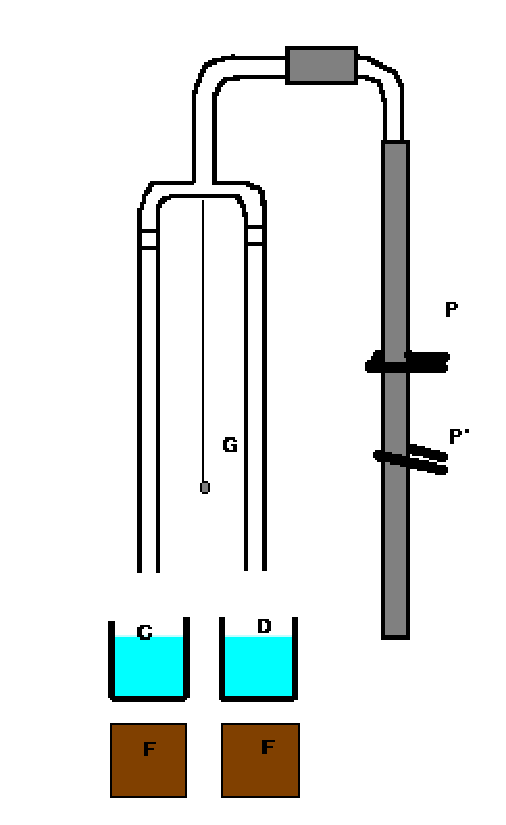
\includegraphics[width=5cm]{hare.eps}
\caption{ヘアの装置}
\label{Hare}
\end{center}
\end{figure}
実際にはビーカー内の液面の位置は測定しにくいので次のようにする。まず目盛り付きのガラス管のなるべく上部まで液体を吸い上げ、液面の位置$h_1$、$h_{1}'$を読み取る。
次になるべく下まで液面を下げ液面の位置$h_2$、$h_{2}'$、\Equref{Hare:kai}より試料密度$\rho$を求める。
\begin{eqnarray}
\label{Hare:kai}
\rho_0 g(h_1-h_2) = \rho g (h_{1}'-h_{2}') すなわち \rho = \frac{h_1-h_2}{h_{1}'-h_{2}'}\rho_0
\end{eqnarray}
なおここでの測定精度を考えると、室温における水の密度$\rho_0$は$1.00\mathrm{g/cm^3}$と近似して良い。
\subsection{通過時刻の測定}
\begin{enumerate}
\item 毛細管に試料液体を吸い上げる\\
※注意
\begin{itemize}
\item 途中に泡が生じたり、液柱が分断されることのないようにゆっくりと吸い上げる。
\item 液を毛細管上端に付いているビニール管内に吸い込ませないようにい注意すること。
\item 水とアルコールを混合させると発熱するため、調合直後の水温が室温に比べ大きく違う場合は数分待って室温に近づけてから実験を行う。
\item 試料液体を変えた場合に、毛細管内部が前回の試料で濡れているため、最初に吸い上げた試料液体は捨てること。
\end{itemize}
\item 毛細管内を大気圧に戻し、液頭が標線を横切っていく時刻を読み取る。実際にはラップタイムが計測できるストップウォッチを使用し、標線を横切る時間をラップタイムで計測する。
\item 液頭の降下が止まったら、毛細管下端から液頭までの高さ(最終停止位置$l_0$)を測る。標線$i$を通過した時刻$T_i$を表にまとめる。
\item $T_i$と下端から標線までの距離$L_i$、$\Delta L_i=L_i-L_{i+1}$とすると、区間の平均速度$v$は以下のように表される。
\begin{eqnarray}
\label{avr-v}
v_i=\frac{L_i-L_{i+1}}{T_{i+1}-T_i}=\frac{\Delta L_i}{\Delta T_i}
\end{eqnarray}
各区間の平均速度$v_i$を縦軸に、その区間の平均点$l_i=(L_i+L_{i+1})/2$の逆数を横軸にとりグラフに表す。
\item 測定は各試料液体につき2,3回繰り返す。
\item すべての測定を終えたら、毛細管内に純粋なアルコールを上端近くまで吸い上げて吐き出す作業を数回繰り返し内部を洗浄、最後に空気を流し乾燥させておく。
\end{enumerate}
\section{結果}
毛細管の型番、測定データは\Tabref{mousai}のようになった
\begin{table}[h]
\caption{型番DE-07,半径$1.686\pm0.002 \times 10^{-9}[\mathrm m]$}
\label{mousai}
\begin{center}
\begin{tabular}{|c|c|c|}\hline
$L_i\mathrm{[cm]}$ & $\Delta L_i\mathrm{[cm]}$ & $1/l_i\mathrm{[cm^{-1}]}$ \\ \hline \hline
96.4& & \\ \hline
87.3& 9.1& 0.011 \\ \hline
78.3& 9.0& 0.012 \\ \hline
69.6& 8.7& 0.014 \\ \hline
61.3& 8.3& 0.015 \\ \hline
53.4& 7.9& 0.017 \\ \hline
45.7& 7.7& 0.020 \\ \hline
38.0& 7.7& 0.023 \\ \hline
33.0& 5.0& 0.028 \\ \hline
28.0& 5.0& 0.033 \\ \hline
23.4& 4.6& 0.039 \\ \hline
18.5& 4.9& 0.048 \\ \hline
13.8& 4.7& 0.062 \\ \hline
8.5& 5.3& 0.090 \\ \hline
4.4& 4.1& 0.016 \\ \hline
\end{tabular}
\end{center}
\end{table}
試料溶液はそれぞれ約25%、50%、75%のものを使用した。計測時の気温は19.4℃、湿度38.7%、気圧1010.5[hPa]となっている。
台の角度$\theta$は61°に設定した。
\begin{itemize}
\item 25%溶液

25%溶液はヘアの装置を用い測定したところ、$h_1=45.8\mathrm{[cm]}$,$h_{1}'=46.8\mathrm{[cm]}$,
$h_2=14.8\mathrm{[cm]}$,$h_{2}'=15.2\mathrm{[cm]}$より、$\rho=0.981\mathrm{[g/cm^3]}$となった。
粘性率の測定結果は以下\Tabref{25-1}から\Tabref{25-3}までとなった。
グラフは巻末図5のようになった。
\begin{table}[h]
\begin{tabular}{cc}
\begin{minipage}{.5\hsize}
\begin{center}
\caption{25%アルコール溶液1回目 $l_s=10.5[\mathrm{cm}]$}
\label{25-1}
\begin{tabular}{|c|c|c|} \hline
  $T_i[\mathrm s]$ & $\Delta T_i[\mathrm s]$ & $v_i=\Delta L_i/\Delta T_i\mathrm{[cm/s]}$ \\ \hline \hline
  0&&\\\hline
  13.55&13.55&0.6716 \\ \hline
  26.81&13.26&0.6787 \\ \hline
  39.64&12.83&0.6780 \\ \hline
  52.30&12.66&0.6556 \\ \hline
  64.94&12.60&0.6270 \\ \hline
  77.62&12.72&0.6053 \\ \hline
  91.28&13.66&0.5637 \\ \hline
  100.8&9.52&0.5252  \\ \hline
  111.1&10.30&0.4854  \\ \hline
  121.5&10.40&0.4423  \\ \hline
  135.3&13.80&0.3551  \\ \hline
  155.0&19.90&0.2362  \\ \hline
\end{tabular}
\end{center}
\end{minipage}
\begin{minipage}{.5\hsize}
\begin{center}
\caption{25%アルコール溶液2回目 $l_s=10.5[\mathrm{cm}]$}
\label{25-2}
\begin{tabular}{|c|c|c|} \hline
  $T_i[\mathrm s]$ & $\Delta T_i[\mathrm s]$ & $v_i=\Delta L_i/\Delta T_i\mathrm{[cm/s]}$ \\ \hline \hline
  0&&\\\hline
  13.60&13.60&0.6691 \\ \hline
  26.73&13.13&0.6855 \\ \hline
  39.49&12.76&0.6818 \\ \hline
  51.92&12.43&0.6677 \\ \hline
  64.49&12.57&0.6285 \\ \hline
  76.96&12.47&0.6175 \\ \hline
  90.51&13.55&0.5683 \\ \hline
  99.81&9.30&0.5376 \\ \hline
  110.0&10.79&0.4634 \\ \hline
  120.4&9.82&0.4684 \\ \hline
  134.2&13.74&0.3566 \\ \hline
  153.9&19.76&0.2379 \\ \hline
\end{tabular}
\end{center}
\end{minipage}
\end{tabular}
\begin{minipage}{.5\hsize}
\begin{center}
\caption{25%アルコール溶液3回目 $l_s=10.4[\mathrm{cm}]$}
\label{25-3}
\begin{tabular}{|c|c|c|} \hline
  $T_i[\mathrm s]$ & $\Delta T_i[\mathrm s]$ & $v_i=\Delta L_i/\Delta T_i\mathrm{[cm/s]}$ \\ \hline \hline
  0&&\\\hline
  13.37&13.37&0.6806 \\ \hline
  26.48&13.11&0.6865 \\ \hline
  39.06&12.56&0.6927 \\ \hline
  51.42&12.36&0.6715 \\ \hline
  63.76&12.34&0.6402 \\ \hline
  76.10&12.34&0.6240 \\ \hline
  89.45&13.35&0.5768 \\ \hline
  98.73&9.28&0.5388 \\ \hline
  108.9&10.19&0.4907 \\ \hline
  118.8&9.91&0.4642 \\ \hline
  132.4&13.62&0.3598 \\ \hline
  151.3&18.86&0.2492 \\ \hline
\end{tabular}
\end{center}
\end{minipage}
\end{table}
\item 50%溶液

 50%溶液はヘアの装置を用い測定したところ、$h_1=41.6\mathrm{[cm]}$,$h_{1}'=44.3\mathrm{[cm]}$,
$h_2=13.3\mathrm{[cm]}$,$h_{2}'=13.9\mathrm{[cm]}$より、$\rho=0.931\mathrm{[g/cm^3]}$となった。
粘性率の測定結果は以下\Tabref{50-1}から\Tabref{50-3}までとなった。
グラフは巻末図6のようになった。
 
\begin{table}[h]
\begin{tabular}{cc}
\begin{minipage}{.5\hsize}
\begin{center}
\caption{50%アルコール溶液1回目 $l_s=8.7[\mathrm{cm}]$}
\label{50-1}
\begin{tabular}{|c|c|c|} \hline
  $T_i[\mathrm s]$ & $\Delta T_i[\mathrm s]$ & $v_i=\Delta L_i/\Delta T_i\mathrm{[cm/s]}$ \\ \hline \hline
  0&&\\\hline
19.92&19.92&0.4568\\\hline
38.98&19.06&0.4722\\\hline
57.08&18.10&0.4807\\\hline
64.54&17.46&0.4754\\\hline
91.84&17.30&0.4566\\\hline
108.9&17.08&0.4508\\\hline
127.1&18.18&0.4235\\\hline
139.5&12.36&0.4045\\\hline
152.9&13.41&0.3728\\\hline
166.0&13.14&0.3501\\\hline
182.3&16.36&0.2995\\\hline
202.6&20.27&0.2319\\\hline
\end{tabular}
\end{center}
\end{minipage}
\begin{minipage}{.5\hsize}
\begin{center}
\caption{50%アルコール溶液2回目 $l_s=8.4[\mathrm{cm}]$}
\label{50-2}
\begin{tabular}{|c|c|c|} \hline
  $T_i[\mathrm s]$ & $\Delta T_i[\mathrm s]$ & $v_i=\Delta L_i/\Delta T_i\mathrm{[cm/s]}$ \\ \hline \hline
  0&&\\\hline
19.43&19.43&0.4683\\\hline
37.88&18.45&0.4878\\\hline
55.35&17.47&0.4980\\\hline
72.41&17.06&0.4865\\\hline
89.46&17.05&0.4633\\\hline
105.9&16.45&0.4680\\\hline
123.7&17.78&0.4330\\\hline
135.7&11.97&0.4177\\\hline
148.7&13.06&0.3828\\\hline
161.2&12.49&0.3683\\\hline
177.1&15.90&0.3082\\\hline
196.5&19.45&0.2416\\\hline
\end{tabular}
\end{center}
\end{minipage}
\end{tabular}
\begin{minipage}{.5\hsize}
\begin{center}
\caption{50%アルコール溶液3回目 $l_s=8.3[\mathrm{cm}]$}
\label{50-3}
\begin{tabular}{|c|c|c|} \hline
  $T_i[\mathrm s]$ & $\Delta T_i[\mathrm s]$ & $v_i=\Delta L_i/\Delta T_i\mathrm{[cm/s]}$ \\ \hline \hline
  0&&\\\hline
  18.16&18.16&0.5011\\\hline
36.06&17.90&0.5028\\\hline
53.16&17.10&0.5088\\\hline
69.91&16.75&0.4955\\\hline
86.56&16.65&0.4745\\\hline
102.9&16.36&0.4707\\\hline
120.3&17.34&0.4440\\\hline
132.2&11.96&0.4181\\\hline
144.9&12.72&0.3931\\\hline
157.2&12.25&0.3755\\\hline
172.9&15.70&0.3121\\\hline
191.2&18.33&0.2564\\\hline
\end{tabular}
\end{center}
\end{minipage}
\end{table}

\item 75%溶液

75%溶液はヘアの装置を用い測定したところ、$h_1=38.6\mathrm{[cm]}$,$h_{1}'=46.0\mathrm{[cm]}$,
$h_2=8.0\mathrm{[cm]}$,$h_{2}'=9.0\mathrm{[cm]}$より、$\rho=0.827\mathrm{[g/cm^3]}$となった。
粘性率の測定結果は以下\Tabref{75-1}から\Tabref{75-3}までとなった。
グラフは巻末図7となった。

\begin{table}[h]
\begin{tabular}{cc}
\begin{minipage}{.5\hsize}
\begin{center}
\caption{75%アルコール溶液1回目 $l_s=7.5\mathrm{cm}]$}
\label{75-1}
\begin{tabular}{|c|c|c|} \hline
  $T_i[\mathrm s]$ & $\Delta T_i[\mathrm s]$ & $v_i=\Delta L_i/\Delta T_i\mathrm{[cm/s]}$ \\ \hline \hline
  0&&\\\hline
  13.99&13.99&0.5011\\\hline
27.86&13.87&0.5028\\\hline
41.11&13.25&0.5088\\\hline
54.01&12.90&0.4955\\\hline
66.86&12.85&0.4745\\\hline
71.48&4.62&0.4707\\\hline
92.86&21.38&0.4441\\\hline
102.0&9.12&0.4181\\\hline
111.6&9.62&0.3931\\\hline
121.0&9.38&0.3755\\\hline
133.2&12.2&0.3121\\\hline
147.1&13.93&0.2564\\\hline
177.0&30.00&0.1767\\\hline
\end{tabular}
\end{center}
\end{minipage}
\begin{minipage}{.5\hsize}
\begin{center}
\caption{75%アルコール溶液2回目 $l_s=7.6[\mathrm{cm}]$}
\label{75-2}
\begin{tabular}{|c|c|c|} \hline
  $T_i[\mathrm s]$ & $\Delta T_i[\mathrm s]$ & $v_i=\Delta L_i/\Delta T_i\mathrm{[cm/s]}$ \\ \hline \hline
  0&&\\\hline
  13.14&13.14&0.6925\\\hline
27.21&13.57&0.6632\\\hline
40.52&13.51&0.6536\\\hline
53.53&13.01&0.6380\\\hline
66.31&12.78&0.6182\\\hline
78.84&12.53&0.6145\\\hline
92.56&13.72&0.5612\\\hline
101.5&9.01&0.5549\\\hline
111.3&9.68&0.5165\\\hline
120.7&9.41&0.4888\\\hline
132.2&11.52&0.4253\\\hline
145.6&13.46&0.3492\\\hline
175.2&29.57&0.1792\\\hline
\end{tabular}
\end{center}
\end{minipage}
\end{tabular}
\begin{minipage}{.5\hsize}
\begin{center}
\caption{75%アルコール溶液3回目 $l_s=7.6[\mathrm{cm}]$}
\label{75-3}
\begin{tabular}{|c|c|c|} \hline
  $T_i[\mathrm s]$ & $\Delta T_i[\mathrm s]$ & $v_i=\Delta L_i/\Delta T_i\mathrm{[cm/s]}$ \\ \hline \hline
  0&&\\\hline
  14.34&14.34&0.6346\\\hline
28.18&13.84&0.6502\\\hline
41.74&13.56&0.6416\\\hline
54.71&12.97&0.6399\\\hline
67.66&12.95&0.6100\\\hline
80.40&12.74&0.6044\\\hline
93.87&13.47&0.5716\\\hline
103.1&9.24&0.5411\\\hline
112.8&9.73&0.5139\\\hline
122.4&9.53&0.4827\\\hline
133.7&11.37&0.4310\\\hline
147.7&14.00&0.3357\\\hline
196.8&29.08&0.1823\\\hline
\end{tabular}
\end{center}
\end{minipage}
\end{table}

\end{itemize}
\section{考察}
図5、図6、図7と\Equref{gamma},\Equref{eta}より、各濃度における$\eta$、$\gamma$を算出したところ、\Tabref{kousatu}のようになった。
\begin{table}[h]
\begin{center}
\caption{各濃度における$\eta$、$\gamma$}
\label{kousatu}
\begin{tabular}{|c|c|c|}\hline
濃度& $\gamma$ & $\eta$ \\ \hline \hline
  25%& $4.49 \times 10^{-8}$ & $1.861 \times 10^{-18}$ \\ \hline
  50%& $2.58 \times 10^{-8}$ & $2.757 \times 10^{-18}$ \\ \hline
  75%& $2.93 \times 10^{-8}$ & $1.485 \times 10^{-18}$ \\ \hline
\end{tabular}
\end{center}
\end{table}

\end{document}
